\chapter{From a scientific question to an access contract}\label{entry:start}

A scientist sees records, intervenes on a system, and tries to infer a property that is not directly visible. The property might be the direction of a microscopic current, an error mechanism in a quantum device, a biochemical turnover rate, or the power consumed by an inaccessible process. The same difficulty appears in each case: different underlying mechanisms can generate the same accessible evidence.

This reference develops a common way to reason about that difficulty. Its subject is \emph{constructive access}: the relation between a specified scientific target, the physical experiments permitted by an apparatus, the distinctions those experiments preserve, and the precision and resources needed to resolve them. ``Constructive'' means that a positive result should provide a usable experiment or decision procedure, and a negative result should identify a reproducible obstruction. The name describes the synthesis developed here. It does not assert that a separate academic field has already been established.

The organizing question is simple:
\begin{quote}
Given these candidate mechanisms and this apparatus, what can we infer about the property we care about, and what would change that answer?
\end{quote}
An answer requires more than a mechanism model. It requires the preparation, controls, recorded outcomes, allowed order of operations, calibration uncertainty, decision objective, and physical resource ledger. Together these form an \emph{access contract}. Every guarantee in the reference is conditional on an explicit contract.

\section{The outcome scientists should expect}
The framework supports four useful outcomes. An \emph{obstruction} proves that a specified distinction is absent from every experiment in the stated access class. A \emph{witness} supplies an experiment whose possible records have different probabilities under the proposed mechanisms. A \emph{precision certificate} establishes how calibration and sampling affect a target estimate or decision. A \emph{resource certificate} bounds a specifically defined expenditure under a justified physical model. These outcomes fit together, but none substitutes for the others.

For example, a nonzero probability contrast proves that information exists in principle. It does not mean a single record determines the answer. A protocol that uses the fewest control actions may require many repetitions. A low dissipation estimate for a visible subsystem does not bound an unobserved fuel-consuming subsystem. A confidence set that retains one target does not establish that the proposed model family includes the real apparatus.

These distinctions make the framework useful across fields: the logical guarantees transfer, while the physical assumptions remain visible.

\section{A first complete example}
The initial example below introduces the access contract with two finite
candidate mechanisms. Later, Chapter~\ref{sec:physical-pulse} moves beyond
that finite dictionary: its response-sign theorem covers every finite
classical network satisfying a local physical intervention contract.
Chapter~\ref{sec:quantum-pulse} derives a quantum response boundary, and
Chapter~\ref{completion:statistics} makes it a finite-data test.
Chapters~\ref{ch:graph-access}--\ref{completion:composition} address the
additional sensors, precision, energy and interfaces needed for broader use.
Chapters~\ref{rr:reset-boundary} and~\ref{rr:explanation} quantify how imperfect resetting and hidden crossing rates can explain a response, including a complete counts-to-confidence calculation. These are different layers of one inference argument. No layer infers the
physical validity of another layer's assumptions merely from a matrix input.

Consider a system with two hidden states, $0$ and $1$. Each experiment starts with probabilities $(1/2,1/2)$. A read operation reports the current state without changing it. Under either candidate mechanism, repeated reads alone produce the same records: all zeros with probability $1/2$, or all ones with probability $1/2$. The mechanisms cannot be distinguished through this access.

Now permit a drive operation. Under mechanism A it replaces the hidden distribution by $(3/4,1/4)$; under mechanism B it replaces it by $(1/4,3/4)$. The drive records only a completion flag. A drive followed by a read gives
\[
 P_A(Y=0)=\frac34,\qquad P_B(Y=0)=\frac14.
\]
The observation has become informative because the permitted experiment changed. No additional processing of the earlier passive records could have produced this distinction.

The complete contract appears in \texttt{examples/active.json}; removing the drive gives \texttt{examples/passive.json}. The two read kernels are
\[
 K^{\mathrm{read},0}=\begin{pmatrix}1&0\\0&0\end{pmatrix},\qquad
 K^{\mathrm{read},1}=\begin{pmatrix}0&0\\0&1\end{pmatrix}.
\]
The drive kernels have identical rows, $(3/4,1/4)$ for A and $(1/4,3/4)$ for B. Kernel entries jointly describe the outcome and the resulting state. This records measurement disturbance whenever it is present; it never discards an inconvenient outcome.

With a read charge of one and drive charge of two, the least action charge of a distinguishing word is three. An independent algebraic checker verifies this claim. Fresh preparation costs an additional modeled unit per record. The complete record distributions have affinity
\[
 \sum_y\sqrt{P_A(y)P_B(y)}=\frac{\sqrt3}{2}.
\]
For equal priors and independent repetitions, the optimal average error is at most half the affinity raised to the record count. Twelve records suffice for the declared $0.1$ average-error target. This is a sufficient count under the specified models; the example does not claim it is the smallest possible count. Its full modeled charge includes twelve preparations as well as twelve drive--read sequences. The unit here is a counted operation, not a joule.

The example already contains the whole research problem: define the distinction, prove why the original access fails, add an allowed intervention, find a witness, compute its actual record law, and account for uncertainty and expenditure. Later chapters replace this small model by continuous-time networks, quantum instruments, and calibrated families of mechanisms.

\begin{figure}[htbp]
\centering
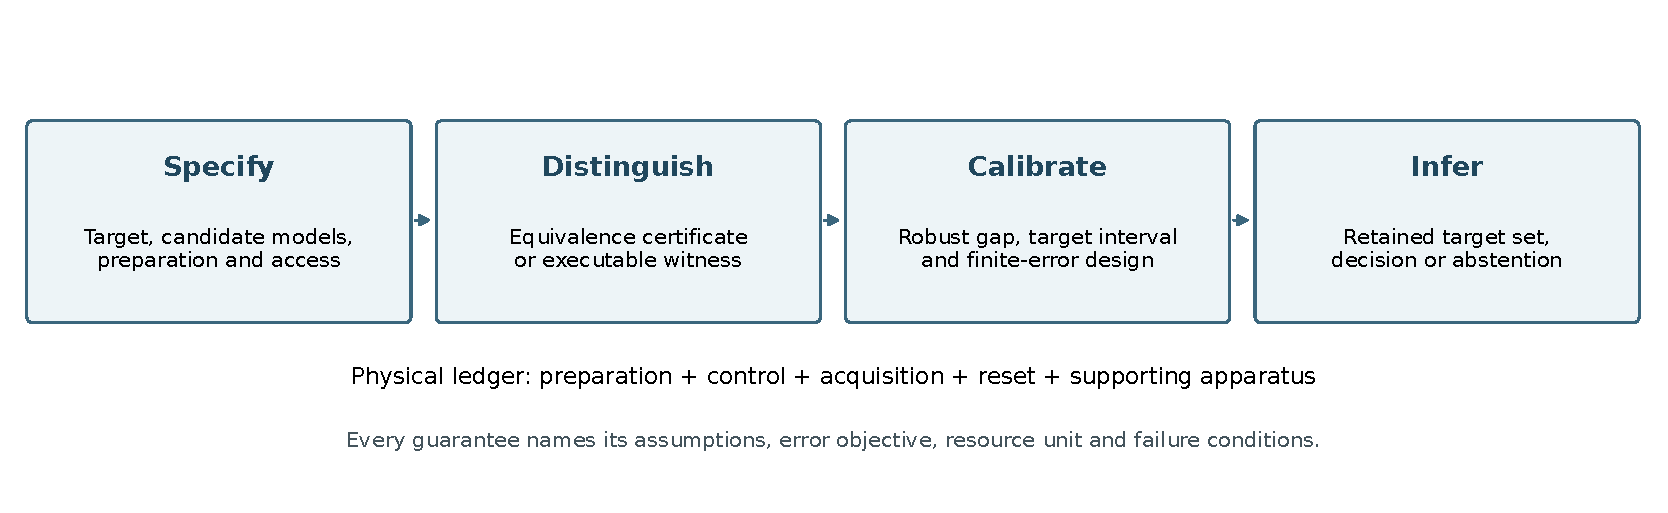
\includegraphics[width=\textwidth]{access_map.pdf}
\caption{The common workflow. Physical assumptions and resource accounting accompany the entire chain, rather than being inferred from a successful algebraic test.}
\label{entry:map}
\end{figure}

\section{A target beyond a supplied list of mechanisms}
The two-state example compares known alternatives. The physical results later
in the reference also bound entire model classes. One example asks how many
hidden classical states are needed to explain two preparation experiments.
Measure their contrast $C_0$ at a common reference time, then measure the same
contrast $C_T$ at a uniformly randomized later time. Under common homogeneous
Markov dynamics and a fixed binary detector, every classical model with at most
three states satisfies $|C_0-C_T|\leq1$, regardless of its unknown rates,
preparation distributions or detector noise. The proof and failure controls
appear in Proposition~\ref{rr:dimension-robust}.

A violation therefore supplies a lower bound on classical realization size.
It does not select a unique replacement model: four classical states can explain
some violating integrated records. This example illustrates the broader
purpose of constructive access. A useful observation can constrain what any
explanation must contain, even when reconstructing the mechanism is impossible.

The extension in Chapter~\ref{rf:entry} asks the same question about larger
classical explanations and physical resources. A finite-data hierarchy forces
at least five classical states in one worked design. A constructive approximation
theorem explains why finite reset records cannot uniformly exclude classical
models of unrestricted size and preparation cost. Stationary correlation
experiments can instead impose dissipation requirements without selecting a
hidden architecture. Together these results identify which added access or
resource premise supports the desired conclusion.

\section{Writing a contract before fitting data}
The following questions specify the experiment rather than merely its interpretation.
\begin{enumerate}
\item \textbf{Target.} What quantity or decision matters? A current's sign, its magnitude, a heat rate, and the full microscopic mechanism are different targets.
\item \textbf{Candidate family.} Which systems remain possible, including nuisance parameters, unknown preparations and detector effects? A nuisance parameter fixed for an entire experiment must stay fixed when calculating its joint record law.
\item \textbf{Preparation.} What can be reset, sampled or conditioned on? A stationary initial distribution is a substantive premise. Independent repetitions require a justified reset or sampling mechanism.
\item \textbf{Operations.} Which controls and measurements can actually be performed, in what order, with what feedback and stopping rules? Unavailable controls do not belong in the witness search.
\item \textbf{Record.} What is retained, including time stamps, failed detections, aborts, and control outcomes? Postselection needs its own success probability and resource accounting.
\item \textbf{Calibration.} Which complete instrument or record laws are bounded, with what joint confidence? Matching one output marginal does not calibrate hidden-state updates.
\item \textbf{Error objective.} Is the goal a worst-case interval, an equal-prior decision error, a posterior risk, or an anytime error guarantee? These objectives need different proofs.
\item \textbf{Resources.} Which contributions to time, gross work, net dissipation, calls or storage are included? State the budget and its units, together with excluded apparatus contributions.
\end{enumerate}
A useful contract also names a negative control and a condition that would cause the inference to be withheld. The software provides such outcomes directly.

\section{The mathematical structure}
The framework has one common object: the map from a hidden mechanism and a permitted protocol to a probability law of accessible records,
\[
 (\theta,\pi)\longmapsto P_\theta^\pi.
\]
The parameter $\theta$ need not be a scalar. It may represent an entire classical or quantum model. A protocol $\pi$ includes the permitted sequence of preparations, actions, observations and decisions. A target $g(\theta)$ states what the scientist wants to learn.

The questions then have a natural order. First, do two mechanisms generate identical accessible laws? Second, is the target constant across those indistinguishable mechanisms? Third, can a finite experiment reveal a relevant difference? Fourth, does the difference survive calibration and sampling? Finally, can the experiment be executed within the stated physical constraints?

The first two questions make sense for very general systems. Finite constructive algorithms require additional structure. The exact algebraic engine in this reference handles finite-dimensional linear representations, including finite classical instruments and finite quantum instruments. Continuous-time approximations, uncertainty sets, and fixed resource budgets add further assumptions. A general definition is not a universal finite algorithm.

\section{How the reference is organized}
The foundations chapter defines targets, accessible laws and equivalence. Finite access turns these definitions into certificates and witness searches. Precision and design link exact differences to robust intervals, statistical error and bounded policies. Model adequacy and physical expenditure explain how conclusions can be withheld and how resource guarantees can be composed. Continuous thermodynamics connects the abstract language to actual transition channels, current measurements and boundaries. The application chapter works through chemistry, quantum diagnostics, sensing and hidden power.

The workflow chapter adds a finite-family procedure that identifies a shared target even when several mechanisms remain indistinguishable. The toolkit chapter documents installation, contracts and independently checked outputs. The closing research map records where the results came from, their relation to established work, and the measurements needed for adoption.

A reader applying the framework can begin with this chapter, run the small example, then use the relevant physical chapter. A reader evaluating the theory should follow the proofs and the assumption tables before interpreting the numerical results. The packaged source and reproducibility driver make both paths checkable.

\section{Scope and scientific status}
The reference integrates proved finite-model results, established mathematical tools, new software interfaces, exact worked examples and internal adversarial checks. It contains no newly measured biological, materials or hardware dataset. It does not establish a physical law governing arbitrary matter, unrestricted total energy, universal quantum characterization, or autonomous improvement of arbitrary computation.

Its foundational contribution is a disciplined interface between questions that are often treated separately: access, identifiability, intervention, calibration, decisions and physical resources. The interface is useful precisely because a limitation or failure in one layer remains visible in the next. Acceptance as a scientific subject depends on independent use, criticism and successful experiments; those cannot be supplied by a manuscript alone.
